\documentclass[a4paper,12pt]{article}

% Pacchetti necessari
\usepackage[utf8]{inputenc}
\usepackage[T1]{fontenc}
\usepackage{graphicx}
\usepackage[italian]{babel}
\usepackage{geometry}
\usepackage{amsmath} 
\usepackage{float}
\usepackage{eso-pic} % Per aggiungere il logo come sfondo
\usepackage{transparent} % Per gestire la trasparenza
\usepackage[hyperindex, bookmarks=true, colorlinks=true, linkcolor=blue, urlcolor=blue]{hyperref}
\usepackage{subfigure} % per inserire due immagini affiancate o per raggruppare in un unico blocco più immagini


% Margini della pagina
\geometry{a4paper, margin=2.5cm}

% Inserimento logo in bianco e nero con opacità
\newcommand\BackgroundLogo{
    \AddToShipoutPictureBG{
        \AtPageLowerLeft{
            \hspace{-3cm}
            \vspace{-4cm}
            \transparent{0.08}
            
\includegraphics[width=12cm, keepaspectratio]{_assets/logo-universita-bn.png}
        }
    }
}

% Comando per abilitare il logo trasparente
\BackgroundLogo

\begin{document}

% Titolo del documento
\begin{titlepage}
    \centering

    \begin{tabular}{@{}c@{\hspace{0.5cm}}c@{}}
        
        \raisebox{-.5\height}{
\includegraphics[width=4cm]{_assets/logo-dipartimento.png}} \\
    \end{tabular}\\[1cm]
    
    {\LARGE Università degli Studi di Salerno}\\[0.5cm]
    {\Large Dipartimento di Ingegneria dell'Informazione ed Elettrica e Matematica Applicata (DIEM)}\\[2cm]
    {\Huge \textbf{Relazione di progetto}}\\[0.4cm]
    {\Large \textbf{Sviluppo di un modello di regressione lineare su dataset}}\\[1cm]
    {\Large Corso di Statistica Applicata - A.A. 2024/25}\\[2cm]
    \begin{flushright}
        \textbf{Studenti Gruppo 16:}\\[0.2cm]
        Corradomaria Giachetta \\
        Matricola: 0612708054 \\
        Francesco Peluso \\
        Matricola: 0612707469 \\[0.2cm]
        Gerardo Selce \\
        Matricola: 0612707692 \\[0.2cm]
        Anuar Zouhri \\
        Matricola: 0612707505 \\[0.2cm]
        \vspace{1cm}
        \textbf{Docenti:}\\
        Prof. Fabio Postiglione \\ Prof. Paolo Addesso 
    \end{flushright}
    \vfill
    Last update: {\large \today}
\end{titlepage}

% Indice
\tableofcontents
\newpage
\section{Descrizione del dataset fornito}
A completezza del progetto si riporta la descrizione del dataset da analizzare. Il dataset contiene $n=100$ osservazioni, costituite da:

\subsection*{Variabile dipendente}
\textbf{y\_VideoQuality} \quad $\rightarrow$ \quad Qualità percepita del video

Tale indice è immaginato come frutto di una opportuna trasformazione di un punteggio assegnato a un campione di immagini da volontari che compilano un questionario. Esso sarà funzione di diverse caratteristiche proprie dei video, tra cui:

\begin{itemize}
	\item la presenza o meno di rumore;
	\item la presenza o meno di \textit{motion blur};
	\item la nitidezza;
	\item la profondità di campo;
	\item la risoluzione;
	\item le aberrazioni ottiche visibili;
	\item la gamma dinamica;
	\item la fedeltà cromatica.
\end{itemize}

\subsection*{Variabili indipendenti (regressori)}

Sono delle quantità di cui l’operatore ha il controllo (parziale o totale) selezionando:

\begin{itemize}
	\item l’attrezzatura video da utilizzare;
	\item i parametri di ripresa.
\end{itemize}

Rappresentano indici standardizzati:

\begin{itemize}
	\item \texttt{x1\_ISO} \quad $\rightarrow$ \quad ISO (sensibilità del sensore)
	\item \texttt{x2\_FRatio} \quad $\rightarrow$ \quad Rapporto Focale
	\item \texttt{x3\_Time} \quad $\rightarrow$ \quad Tempo di Esposizione (in relazione al frame rate utilizzato)
	\item \texttt{x4\_MP} \quad $\rightarrow$ \quad Megapixel del sensore
	\item \texttt{x5\_CROP} \quad $\rightarrow$ \quad Fattore di Crop
	\item \texttt{x6\_FOCAL} \quad $\rightarrow$ \quad Focale
	\item \texttt{x7\_PixDensity} \quad $\rightarrow$ \quad Densità di pixel
\end{itemize}



\newpage
\section{Analisi delle caratteristiche del dataset}
In questa fase preliminare si illustreranno le principali considerazioni fatte sul dataset fornito.
\subsection{Boxplot dei dati}
Si considerino i seguenti boxplot delle variabili del dataset.
\begin{figure}[h]
	\centering
	\subfigure[Boxplot della variabile dipendente y\_VideoQuality]{
		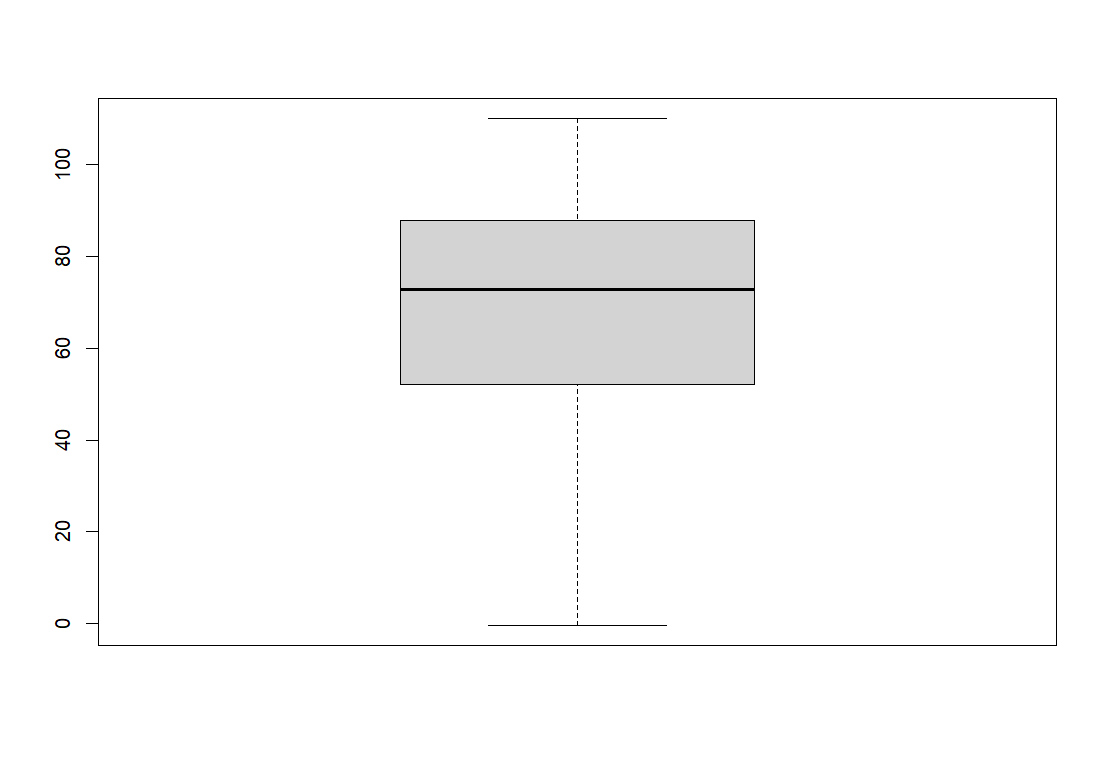
\includegraphics[width=0.65\linewidth]{../graphs/DescriptiveStatisticPlots/boxplot_y_VideoQuality}
		\label{fig:boxplotyvideoquality}
	}
	\subfigure[Boxplot delle variabili indipendenti x\_i]{
		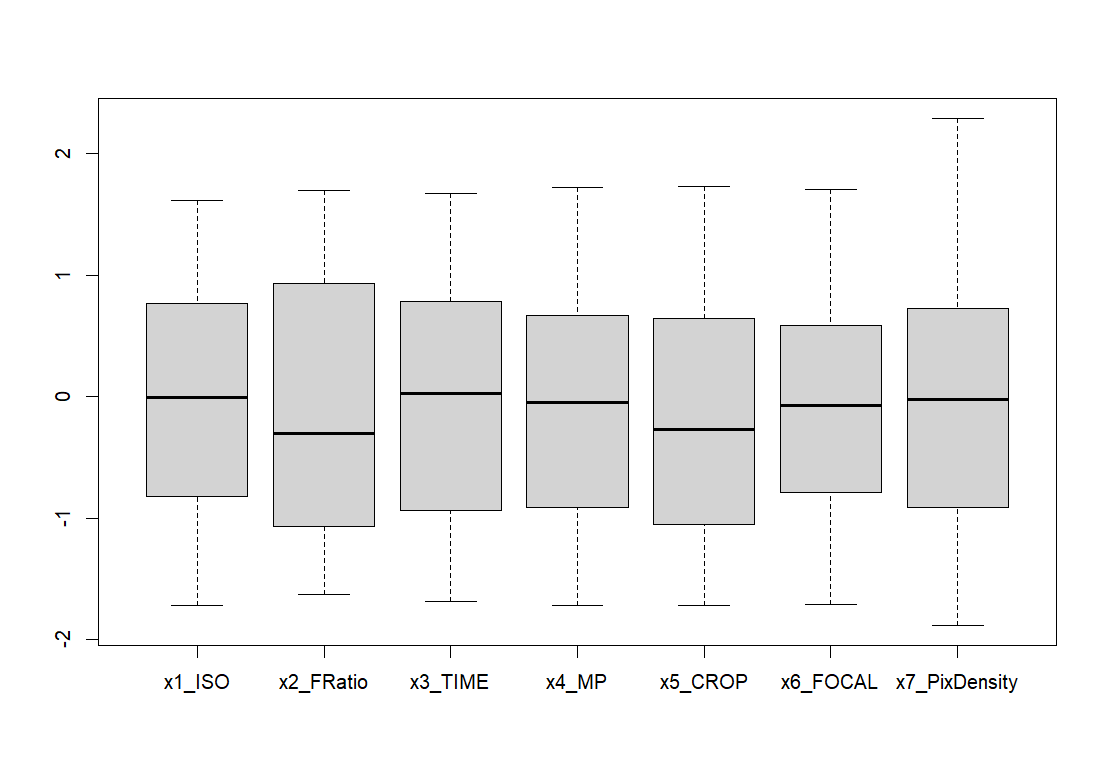
\includegraphics[width=0.65\linewidth]{../graphs/DescriptiveStatisticPlots/boxplot_all_x_i}
		\label{fig:boxplotallxi}
	}
	\caption{Boxplot delle variabili considerate}
\end{figure}

Si osservi innanzitutto che i valori per ciascuna variabile sono tutti contenuti all'interno dell'intervallo interquartile e che quindi non sono presenti outliers. Per quel che riguarda la variabile dipendente y\_VideoQuality si è osservato che il valore della media e della mediana sono simili, infatti valgono rispettivamente  $\text{media}=72.8135, \text{mediana}=68.6081$. Si è osservato inoltre che i valori assunti dalla variabile x7$\_$PixDensity coprono un intervallo maggiore rispetto alle altre variabili indipendenti. 
\subsection{Analisi di normalità}
Anche se non strettamente necessario ai fini del metodo di regressione, si è comunque deciso di verificare se qualcuna delle variabili indipendenti avesse una distribuzione normale.\begin{figure}[h]
	\centering
	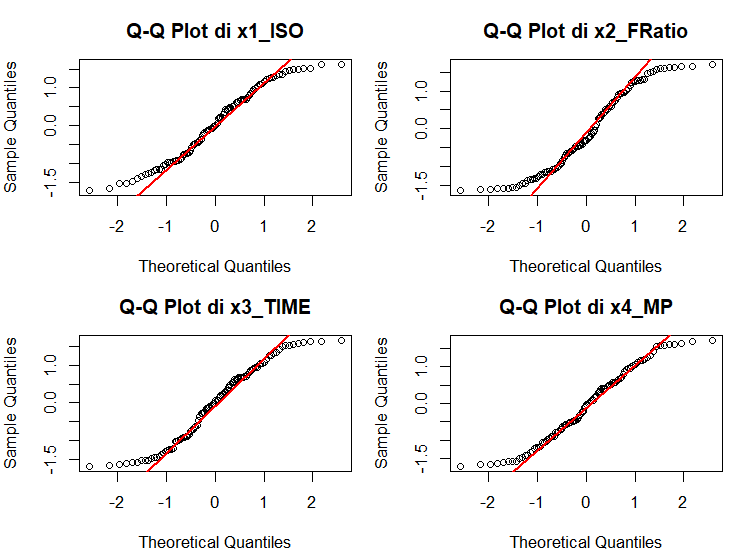
\includegraphics[width=0.9\linewidth]{../graphs/DescriptiveStatisticPlots/qqplot1/qqplot1}
	\caption{}
	\label{fig:qqplot1}
\end{figure}
Tra i diversi qq-plot, si osserva che la variabile x6$\_$Focal sembrerebbe avere una distribuzione normale. Applicando il test di shapiro a questa variabile si ottiene
\begin{align*}
	\text{W} = 0.97, \text{p-value} = 0.02.
\end{align*}
Il valore di p-value ottenuto non si discosta molto da 0.05 e si potrebbe perciò supporre che la variabile sia distribuita come una normale.
\begin{figure}[h]
	\subfigure{
		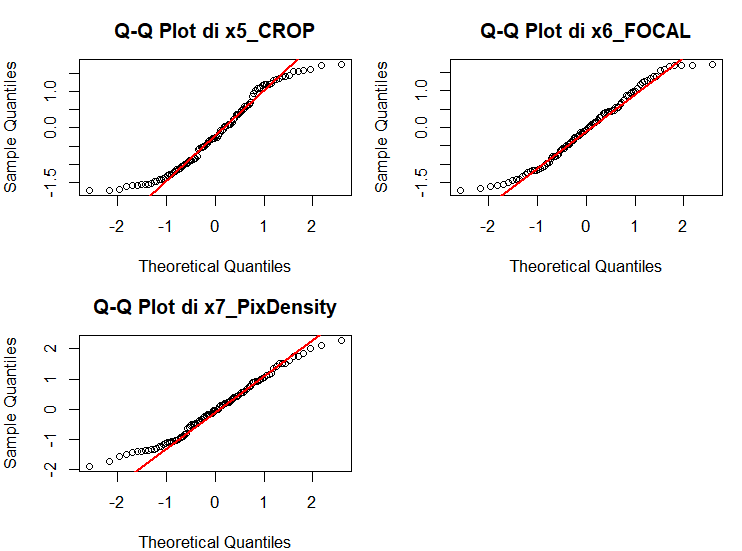
\includegraphics[width=0.9\linewidth]{../graphs/DescriptiveStatisticPlots/qqplot1/qqplot2}
		\label{fig:qqplot2}	
		}
\end{figure}





\newpage
\section{Analisi della dipendenza tra le variabili}


\subsection{Analisi di correlazione}

\begin{figure}[H]
	\centering
	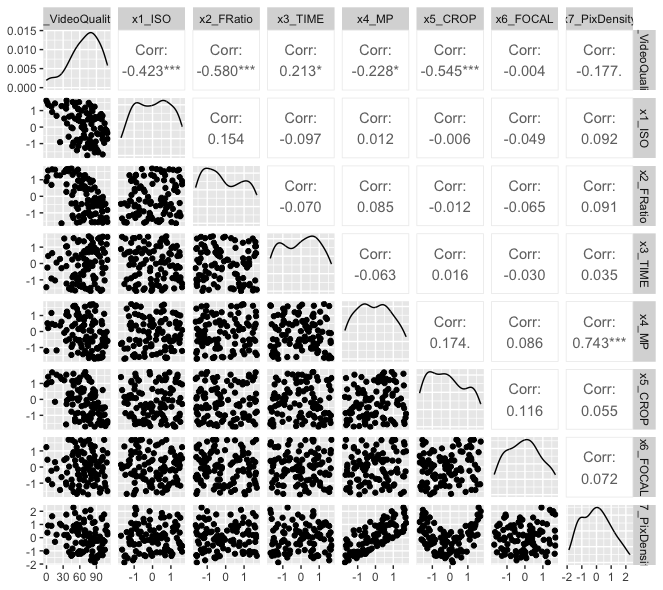
\includegraphics[width=0.90\textwidth]{../graphs/DescriptiveStatisticPlots/ggplot}
	\caption{Scatter plot delle variabili presenti nel dataset.}
\end{figure}

Dalla Figura (3) notiamo, anche dal coefficiente di correlazione, una dipendenza lineare tra le variabili:
\begin{itemize}
	\item \textbf{x4\_MP} e \textbf{x7\_PixDensity}
\end{itemize}
Invece notiamo la presenza di dipendenze non lineari che non vengono descritte dal coefficiente di correlazione. In particolare la notiamo tra le variabili:
\begin{itemize}
	\item \textbf{y\_VideoQuality} e \textbf{x1\_ISO}
	\item \textbf{y\_VideoQuality} e \textbf{x2\_FRatio}
	\item \textbf{y\_VideoQuality} e \textbf{x3\_Time}
	\item \textbf{y\_VideoQuality} e \textbf{x5\_CROP}
	\item \textbf{x5\_CROP} e \textbf{x7\_PixDensity}
\end{itemize}

\subsection{Analisi di regressione}
Le dipendenze tra la variabile y\_VideoQuality e le diverse variabili indipendenti sono state analizzate attraverso una regressione semplice sulle singole variabili indipendenti.
\begin{table}[H]
	\centering
	\begin{tabular}{|c|c|}
		\hline
		\textbf{Variabile indipendente} & \textbf{p-value} \\
		\hline
		x1\_ISO & $1.17e-05$ \\
		\hline
		x2\_FRatio & $2.63e-10$ \\ 
		\hline
		x3\_TIME & $0.0331e$ \\
		\hline
		x4\_MP & $0.0227$ \\
		\hline
		x5\_CROP & $4.39e-09$ \\
		\hline
		x6\_FOCAL & $0.97$ \\
		\hline
		x7\_PixDensity & $0.0775$ \\
		\hline
	\end{tabular}
	\caption{Sono rappresentati i p-value relativi alle regressioni delle singole variabili indipendenti al primo grado.}
	\label{tab:}
\end{table}
Diversamente da quanto ottenuto nell'analisi di correlazione, dalla Tabella (1) risultano rilevanti i regressori x1, x2, x3. La stessa analisi è stata poi effettuata considerando anche i regressori al secondo ordine.

\begin{table}[H]
	\centering
	\begin{tabular}{|c|c|}
		\hline
		\textbf{Variabile indipendente} & \textbf{p-value} \\
		\hline
		x1\_ISO & $2.46e-03$ \\
		\hline
		x2\_FRatio & $1.28e-3$ \\ 
		\hline
		x3\_TIME & $0.3094$ \\
		\hline
		x4\_MP & $0.2899$ \\
		\hline
		x5\_CROP & $0.368$ \\
		\hline
		x6\_FOCAL & $0.770$ \\
		\hline
		x7\_PixDensity & $0.8038$ \\
		\hline
	\end{tabular}
	\caption{Sono rappresentati i p-value relativi alle regressioni delle singole variabili indipendenti al secondo grado.}
	\label{tab:}
\end{table}
Dalla Tabella (2) risulta evidente una dipendenza quadratica della variabile dipendente dai regressori x1, x2.


\newpage
\section{Analisi dei modelli}
In questa sezione si analizzeranno differenti modelli e successivamente li si confronteranno verificando quale dei modelli meglio soddisfa l'ipotesi di normalità dei residui tramite dei grafici e test diagnostici. Inoltre, dato il numero non elevato di campioni si confronteranno i valori di AIC e di adjusted-$R^2$.


\subsection{Modello 1}
Il primo modello analizzato è quello che include i regressori (di primo grado) più significativi (in base al valore di p\_value misurato precedentemente). Ovvero:
\begin{equation*}
y=\beta_0+\beta_1x_1+\beta_2x_2+\beta_3x_3+\beta_5x_5.
\end{equation*}
La stima dei parametri ottenuti per questo modello è
\begin{table}[H]
	\centering
	\begin{tabular}{|c|c|c|}
		\hline
		\textbf{Parametro} & \textbf{Stima} & \textbf{Dev. Std.} \\
		\hline
		$\beta_0$ & 65.62  & 1.30 \\
		$\beta_1$ & -9.37  & 1.38 \\
		$\beta_2$ & -13.33 & 1.24 \\
		$\beta_3$ & 4.01   & 1.26 \\
		$\beta_5$ & -14.52 & 1.26 \\
		\hline
	\end{tabular}
	\caption{Stime dei coefficienti e deviazioni standard del modello}
	\label{tab:coef_estimates}
\end{table}

Gli intervalli di confidenza al $5\%$, ottenuti tramite il metodo confint() di R, sono:
\begin{table}[H]
	\centering
	\begin{tabular}{|c|c|c|}
		\hline
		\textbf{Parametro} & \textbf{Lower bound} & \textbf{Upper bound} \\
		\hline
		$\beta_0$ & 63.04 & 68.20 \\
		$\beta_1$ & -12.11 & -6.62 \\
		$\beta_2$ & -15.79 & -10.87 \\
		$\beta_3$ & 1.51 & 6.51 \\
		$\beta_5$ & -17.01 & -12.03 \\
		\hline
	\end{tabular}
	\caption{Intervalli di confidenza al 95\% per i coefficienti del modello}
	\label{tab:ci_coefficienti}
\end{table}

I valori dell'adjusted $R^2$  e AIC ottenuti sono:
\begin{equation*}
	R^2 =  0.77, \quad AIC = 514.69.
\end{equation*}
\subsection{Modello 2}
Il prossimo modello analizzato è quello ottenuto aggiungendo tutti i regressori più significativi con l'aggiunta di alcuni regressori al quadrato.
\begin{equation*}
	y=\beta_0 + \beta_1x_1+\beta_2x_1^2+\beta_3x_2+\beta_4x_2^2+\beta_5x_3+\beta_6x_5
\end{equation*}
La stima dei parametri ottenuti per questo modello è
\begin{table}[H]
	\centering
	\begin{tabular}{|c|c|c|}
		\hline
		\textbf{Parametro} & \textbf{Stima} & \textbf{Dev. Std.} \\
		\hline
		$\beta_0$ & 79.93  & 1.95 \\
		$\beta_1$ & -8.66  & 1.05 \\
		$\beta_2$ & -8.03  & 1.23 \\
		$\beta_3$ & -13.49 & 0.94 \\
		$\beta_4$ & -6.38  & 1.09 \\
		$\beta_5$ & 3.94   & 0.95 \\
		$\beta_6$ & -13.23 & 0.96 \\
		\hline
	\end{tabular}
	\caption{Stime dei coefficienti e errori standard del modello}
	\label{tab:coef_estimates_poly}
\end{table}

Gli intervalli di confidenza al $5\%$, ottenuti tramite il metodo confint() di R, sono:
\begin{table}[H]
	\centering
	\begin{tabular}{|c|c|c|}
		\hline
		\textbf{Parametro} & \textbf{Lower bound} & \textbf{Upper bound} \\
		\hline
		$\beta_0$ & 76.06 & 83.80 \\
		$\beta_1$ & -10.75 & -6.58 \\
		$\beta_2$ & -10.48 & -5.58 \\
		$\beta_3$ & -15.36 & -11.63 \\
		$\beta_4$ & -8.55 & -4.22 \\
		$\beta_5$ & 2.05 & 5.84 \\
		$\beta_6$ & -15.14 & -11.32 \\
		\hline
	\end{tabular}
	\caption{Intervalli di confidenza al 95\% per i coefficienti del modello}
	\label{tab:ci_coefficienti}
\end{table}

I valori dell'adjusted $R^2$  e AIC ottenuti sono:
\begin{equation*}
	R^2 =   0.87, \quad AIC = 460.76.
\end{equation*}
\subsection{Modello 3}
Questo modello è ottenuto tramite la funzione step() di R eliminando i regressori non significativi, a partire dal modello contenente tutti i regressori di primo grado. Il modello ottenuto è:
\begin{equation*}
	y=\beta_0+\beta_1x_1+\beta_2x_2+\beta_3x_3+\beta_4x_5+\beta_5x_7
\end{equation*}
La stima dei parametri ottenuti per questo modello è:
\begin{table}[H]
	\centering
	\begin{tabular}{|c|c|c|}
		\hline
		\textbf{Parametro} & \textbf{Stima} & \textbf{Dev. Std.} \\
		\hline
		$\beta_0$ & 65.65  & 1.29 \\
		$\beta_1$ & -9.18  & 1.38 \\
		$\beta_2$ & -13.17 & 1.23 \\
		$\beta_3$ & 4.11   & 1.25 \\
		$\beta_4$ & -14.41 & 1.25 \\
		$\beta_5$ & -2.02  & 1.29 \\
		\hline
	\end{tabular}
	\caption{Stime dei coefficienti e deviazioni standard del modello}
	\label{tab:coef_estimates_poly}
\end{table}
Gli intervalli di confidenza al $5\%$, ottenuti tramite il metodo confint() di R, sono:
\begin{table}[H]
	\centering
	\begin{tabular}{|c|c|c|}
		\hline
		\textbf{Parametro} & \textbf{Lower bound} & \textbf{Upper bound} \\
		\hline
		$\beta_0$ & 63.08 & 68.21 \\
		$\beta_1$ & -11.92 & -6.45 \\
		$\beta_2$ & -15.62 & -10.72 \\
		$\beta_3$ & 1.62 & 6.59 \\
		$\beta_4$ & -16.89 & -11.93 \\
		$\beta_5$ & -4.58 & 0.54 \\
		\hline
	\end{tabular}
	\caption{Intervalli di confidenza al 95\% per i coefficienti del modello}
	\label{tab:ci_coefficienti}
\end{table}
I valori dell'adjusted $R^2$  e AIC ottenuti sono:
\begin{equation*}
	R^2 =    0.77, \quad AIC =  514.11.
\end{equation*}
\subsection{Modello 4}
L'ultimo modello analizzato, è ottenuto tramite la seguente istruzione R, adottando la funzione step():
\begin{align*}
	y &= \beta_0 
	+ \beta_1 x_1 + \beta_2 x_2 + \beta_3 x_3 + \beta_4 x_4 + \beta_5 x_5 
	+ \beta_6 x_6 + \beta_7 x_7 
	+ \beta_8 x_1^2 + \beta_9 x_2^2 + \beta_{10} x_6^2 + \beta_{11} x_7^2 \\
	&+ \beta_{12} x_1 x_6 + \beta_{13} x_2 x_4 + \beta_{14} x_3 x_4 
	+ \beta_{15} x_3 x_5 + \beta_{16} x_3 x_7 
	+ \beta_{17} x_4 x_7.
\end{align*}
In particolare il modello di partenza da cui si è partiti:
\begin{verbatim}
	model_step_interactions <- lm(y_VideoQuality ~ (.)^2 + I(x1_ISO^2) + 
	I(x2_FRatio^2) + I(x3_TIME^2) + I(x4_MP^2) + I(x5_CROP^2) + I(x6_FOCAL^2) + 
	I(x7_PixDensity^2), data = data)
\end{verbatim}
La stima dei parametri ottenuti per questo modello è:
\begin{table}[H]
	\centering
	\begin{tabular}{|c|c|c|}
		\hline
		\textbf{Parametro} & \textbf{Stima} & \textbf{Dev. Std.} \\
		\hline
		$\beta_0$   & 81.64  & 2.18 \\
		$\beta_1$   & -8.77  & 1.00 \\
		$\beta_2$   & -13.56 & 0.90 \\
		$\beta_3$   & 4.31   & 1.03 \\
		$\beta_4$   & -0.25  & 1.46 \\
		$\beta_5$   & -13.37 & 0.92 \\
		$\beta_6$   & 0.62   & 0.99 \\
		$\beta_7$   & -2.96  & 1.60 \\
		$\beta_8$   & -8.85  & 1.16 \\
		$\beta_9$   & -6.57  & 1.01 \\
		$\beta_{10}$ & -1.89  & 1.07 \\
		$\beta_{11}$ & 2.91   & 1.86 \\
		$\beta_{12}$ & -1.71  & 1.18 \\
		$\beta_{13}$ & 1.66   & 0.99 \\
		$\beta_{14}$ & -2.81  & 1.42 \\
		$\beta_{15}$ & 2.83   & 0.99 \\
		$\beta_{16}$ & 3.24   & 1.54 \\
		$\beta_{17}$ & -3.55  & 2.25 \\
		\hline
	\end{tabular}
	\caption{Stime dei coefficienti e deviazioni standard del modello}
	\label{tab:stima_coef_std}
\end{table}
Gli intervalli di confidenza al $5\%$, ottenuti tramite il metodo confint() di R, sono:
\begin{table}[H]
	\centering
	\begin{tabular}{|c|c|c|}
		\hline
		\textbf{Parametro} & \textbf{Lower bound} & \textbf{Upper bound} \\
		\hline
		$\beta_0$   & 77.29  & 85.99 \\
		$\beta_1$   & -10.76 & -6.78 \\
		$\beta_2$   & -15.34 & -11.77 \\
		$\beta_3$   & 2.26   & 6.37 \\
		$\beta_4$   & -3.16  & 2.65 \\
		$\beta_5$   & -15.20 & -11.53 \\
		$\beta_6$   & -1.34  & 2.59 \\
		$\beta_7$   & -6.14  & 0.22 \\
		$\beta_8$   & -11.16 & -6.55 \\
		$\beta_9$   & -8.58  & -4.57 \\
		$\beta_{10}$ & -4.01  & 0.23 \\
		$\beta_{11}$ & -0.78  & 6.61 \\
		$\beta_{12}$ & -4.05  & 0.64 \\
		$\beta_{13}$ & -0.31  & 3.62 \\
		$\beta_{14}$ & -5.65  & 0.02 \\
		$\beta_{15}$ & 0.86   & 4.81 \\
		$\beta_{16}$ & 0.19   & 6.30 \\
		$\beta_{17}$ & -8.02  & 0.93 \\
		\hline
	\end{tabular}
	\caption{Intervalli di confidenza al 95\% per i coefficienti del modello}
	\label{tab:ci_coefficienti}
\end{table}
I valori dell'adjusted $R^2$  e AIC ottenuti sono:
\begin{equation*}
	R^2 =      0.89, \quad AIC=448.27.
\end{equation*}




\end{document}
